\begin{figure}
  \centering
  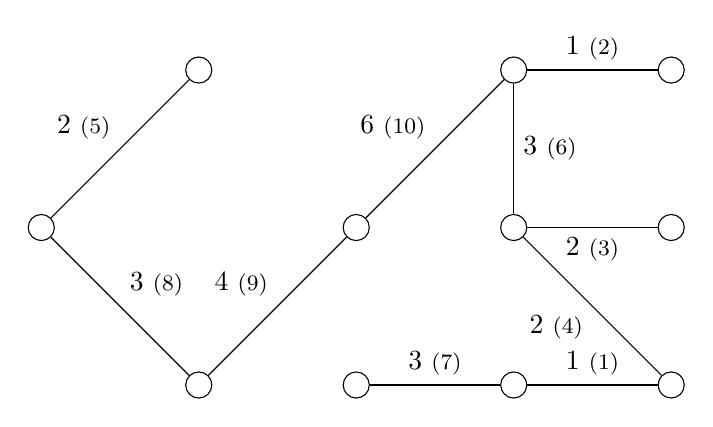
\begin{tikzpicture}[auto, node distance=2cm, main node/.style={circle, draw, minimum size=.5em}]
    \node[main node] (0) {};
    \node[main node] (1) [right of=0, below of=0] {};
    \node[main node] (2) [above of=1, above of=1] {};
    \node[main node] (3) [right of=2, below of=2] {};
    \node[main node] (4) [right of=3, above of=3] {};
    \node[main node] (5) [right of=4] {};
    \node[main node] (6) [below of=3] {};
    \node[main node] (7) [right of=6] {};
    \node[main node] (8) [right of=7] {};
    \node[main node] (9) [above of=8] {};
    \node[main node] (10) [left of=9] {};

    \path[every node]
    (7) edge node {1 \footnotesize{(1)}} (8)
    (4) edge node {1 \footnotesize{(2)}} (5)
    (9) edge node {2 \footnotesize{(3)}} (10)
    (8) edge node {2 \footnotesize{(4)}} (10)
    (0) edge node {2 \footnotesize{(5)}} (2)
    (4) edge node {3 \footnotesize{(6)}} (10)
    (6) edge node {3 \footnotesize{(7)}} (7)
    (0) edge node {3 \footnotesize{(8)}} (1)
    (1) edge node {4 \footnotesize{(9)}} (3)
    (3) edge node {6 \footnotesize{(10)}} (4)
    ;
  \end{tikzpicture}

  \caption{ein möglicher MST}\label{fig:kruskalmst}
\end{figure}